\begin{frame}
\frametitle{Area of Interest in Bavaria}
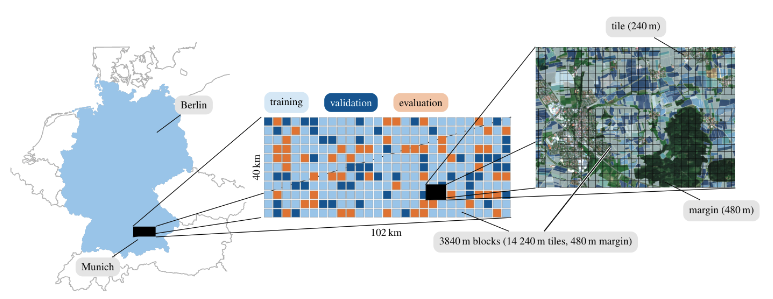
\includegraphics[width=\textwidth]{images/aoi}
%\tikzstyle{annotation} = [fill=tumgraylight, rounded corners]

\tikzset{pic shift/.store in=\shiftcoord,
	pic shift={(0,0)},
	tcube/.pic = {
		%%% small temporal cube showing multitemporal observations %%%
		
		\begin{scope}[perspective3d, node distance=.8em]
			
			\def\size{3em}
			\def\d{.3}
			
			\node[fill=tumwhite, transform shape, canvas is yx plane at z=0*\d] (bottom) {\includegraphics[width=\size,height=\size]{images/tiles480/20160212}};
			\node[right=of bottom.east]{$t_{4}$};
			
			\node[fill=tumwhite, transform shape, canvas is yx plane at z=1*\d] (mid1) {\includegraphics[width=\size,height=\size]{images/tiles480/20160522}};
			\node[right=of mid1.east]{$t_{15}$};
			
			\node[fill=tumwhite, transform shape, canvas is yx plane at z=2*\d] (mid2) {\includegraphics[width=\size,height=\size]{images/tiles480/20160628}};
			\node[right=of mid2.east]{$t_{19}$};
			
			\node[fill=tumwhite, transform shape, canvas is yx plane at z=3*\d] (mid3) {\includegraphics[width=\size,height=\size]{images/tiles480/20160820}};
			\node[right=of mid3.east]{$t_{28}$};
			
			\node[fill=tumwhite, transform shape, canvas is yx plane at z=4*\d] (top) {\includegraphics[width=\size,height=\size]{images/tiles480/20160912}};
			\node[right=of top.east]{$t_{32}$};
			
			%\foreach \i in {south west, south east, north east, north west}
			%\draw[dashed] (bottom.\i) -- (top.\i) coordinate(b-\i);
			
			%\draw (b-south west)--(b-south east)--(b-north east)--(b-north west)--cycle;
			
		\end{scope}
	}
}
\tikzset{pic shift/.store in=\shiftcoord,
	pic shift={(0,0)},
	cube/.pic = {
	\begin{scope}[perspective3d]
		
		\def\cubewidth{13em}
		\def\d{.4}
		
		\node[canvas is yx plane at z=0*\d, draw, transform shape] (a) {\includegraphics[width=\cubewidth]{images/aoi/backgroundS2A20160721}};
		\node[canvas is yx plane at z=0*\d, transform shape, fill opacity=.2]{\resizebox{\cubewidth}{!}{\input{images/aoi/zoomed_gridtraintest.tikz}}};
		\node[canvas is yx plane at z=1*\d,draw,transform shape, fill opacity=1]{\resizebox{\cubewidth}{!}{\input{images/aoi/zoomed_480tiles.tikz}}};
		\node[canvas is yx plane at z=2*\d, draw,transform shape, opacity=1]{\resizebox{\cubewidth}{!}{\input{images/aoi/fields.tikz}}};
		
		%		\foreach \i in {south west, south east, north east, north west}
		%		\draw[dashed] (a.\i) --++(0,0,3) coordinate(b-\i);
		%		
		%		\draw (b-south west)--(b-south east)--(b-north east)--(b-north west)--cycle;
		%		
	\end{scope}
	}
}

\tikzset{pic shift/.store in=\shiftcoord,
	pic shift={(0,0)},
	map/.pic = {
	\begin{scope}[y=0.80pt, x=0.80pt, yscale=-0.15, xscale=0.15, inner sep=0pt, outer sep=0pt]
		
		
		\begin{scope}[cm={{0.99907,0.0,0.0,0.99907,(0.0,0.0)}},draw=black!30,line join=bevel,line cap=rect,line width=0.5pt]
			\input{images/aoi/borders.tikz}
		\end{scope}
		
		\begin{scope}[cm={{0.99907,0.0,0.0,0.99907,(0.0,0.0)}},draw=tumbluelight, fill=tumbluelight,line join=bevel,line cap=rect,line width=0.5pt]
			\input{images/aoi/germany.tikz}
		\end{scope}
		
%		\begin{scope}[cm={{0.99907,0.0,0.0,0.99907,(0.0,0.0)}},draw=tumblack,fill=tumblack,line join=bevel,line cap=rect,line width=0.5pt]
%			\input{images/aoi/aoibox.tikz}
%		\end{scope}
		
	\end{scope}
	}
}

\tikzset{pic shift/.store in=\shiftcoord,
	pic shift={(0,0)},
	zoomed/.pic = {
		\begin{scope}[]
			
			\def\boxwidth{13em}
			%\def\d{.4}
			
			\node[] (a) {\includegraphics[width=\boxwidth]{images/aoi/backgroundS2A20160721}};
			\node[fill opacity=.2]{\resizebox{\boxwidth}{!}{\input{images/aoi/zoomed_gridtraintest.tikz}}};
			\node[opacity=1]{\resizebox{\boxwidth}{!}{\input{images/aoi/buffered_tiles.tikz}}};
			%\node[fill opacity=1]{\resizebox{\cubewidth}{!}{\input{images/aoi/zoomed_480tiles.tikz}}};
			\node[opacity=1]{\resizebox{\boxwidth}{!}{\input{images/aoi/fields.tikz}}};
			
			%		\foreach \i in {south west, south east, north east, north west}
			%		\draw[dashed] (a.\i) --++(0,0,3) coordinate(b-\i);
			%		
			%		\draw (b-south west)--(b-south east)--(b-north east)--(b-north west)--cycle;
			%		
		\end{scope}
	}
}
%\tikzset{external/export next=false}
%\tikzsetnextfilename{aoimap}
\begin{tikzpicture}[]

%\node[](aoi) at (0,0){
%	%\begin{tikzpicture}[y=0.80pt, x=0.80pt, yscale=-0.15, xscale=0.15, inner sep=0pt, outer sep=0pt]
%	\begin{scope}[y=0.80pt, x=0.80pt, yscale=-0.15, xscale=0.15, inner sep=0pt, outer sep=0pt]
%	
%	
%	\begin{scope}[cm={{0.99907,0.0,0.0,0.99907,(0.0,0.0)}},draw=black!30,line join=bevel,line cap=rect,line width=0.5pt]
%	\input{images/aoi/borders.tikz}
%	\end{scope}
%	
%	\begin{scope}[cm={{0.99907,0.0,0.0,0.99907,(0.0,0.0)}},draw=tumbluelight, fill=tumbluelight,line join=bevel,line cap=rect,line width=0.5pt]
%	\input{images/aoi/germany.tikz}
%	\end{scope}
%	
%	\begin{scope}[cm={{0.99907,0.0,0.0,0.99907,(0.0,0.0)}},draw=tumblack,fill=tumblack,line join=bevel,line cap=rect,line width=0.5pt]
%	\input{images/aoi/aoibox.tikz}
%	\end{scope}
%	
%	\end{scope}
%	};

\coordinate (map) at (0,0);
\draw pic (aoi) at (map) {map};

%\draw[step=1.0,black,thin] (0,0) grid (5,-5);
\node[rectangle, inner sep=0, minimum width=4.5mm, minimum height=2mm, fill=tumblack, opacity=1] (aoirect) at ($ (map)+(2.15,-3.29) $){};

\coordinate (Berlin) at ($ (map)+(2.4,-1.3) $);
\node[annotation, above right= 5mm of Berlin](annotBerlin){\tiny Berlin};
\draw (Berlin) -- (annotBerlin);

\coordinate (Munich) at ($ (map)+(2.02,-3.45) $);
\node[annotation, below left= 5mm of Munich](annotMunich){\tiny Munich};
\draw (Munich) -- (annotMunich);

% draw relative to aoi node
%\begin{scope}[x={(aoi.south east)},y={(aoi.north west)}]
%\draw[red,ultra thick,rounded corners] (.5,.2) rectangle ++(0,0);
%\end{scope}

\visible<2->{
	\coordinate (A) at (6,-2);
	\node[inner sep=0](fold) at (A){
		\phantom{\resizebox{5cm}{!}{\input{images/aoi/fold0_with_margin.tikz}}}
	};	
	
	\draw (aoirect.south east) -- (fold.south east); 
	\draw (aoirect.south west) -- (fold.south west);
	\draw (aoirect.north east) -- (fold.north east);
	\draw (aoirect.north west) -- (fold.north west);
	
	\node[inner sep=0](fold) at (A){
		\resizebox{5cm}{!}{\input{images/aoi/fold0_with_margin.tikz}}
	};	
	
	\node[rectangle, inner sep=0, minimum width=4mm, minimum height=3mm, fill=tumblack, draw=tumblack, opacity=1] (foldrect) at ($ (fold)+(1,-.5) $){};
	
	\node[below = 1mm of fold](aoiwidth){\tiny \SI{102}{\km}};
	\node[left = 1mm of fold, anchor=center, rotate=90](aiuheight){\tiny \SI{40}{\km}};
	
	\coordinate (training) at ($ (A)+(-2,1.3) $);
	\node[annotation, fill=traincolor!40](annotTrain) at (training){\tiny training};
	\node[annotation, right= 3mm of annotTrain, fill=validcolor, text=white](annotValid){\tiny validation};
	\node[annotation, right= 3mm of annotValid, fill=evalcolor!40](annotEval){\tiny evaluation};

	\node[annotation](annotBlock) at ($ (A)+(3,-1.5) $){\tiny \SI{3840}{\m} blocks (14 \SI{240}{\m} tiles, \SI{480}{\m} margin)};
	
	\draw (annotBlock) -- ($ (A)+(1.52,-.9) $);
}

\visible<3->{
	\coordinate (B) at (11,-1);
	\draw[draw=white, double=black] (annotBlock) -- ($ (B)+(-.5,-.6) $);
	%\draw pic (bigcube) at (0,7,1.5) {zoomed};
	\phantom{\node[inner sep=0] (bigcube) at (B) {\includegraphics[width=4cm]{images/aoi/zoomed.pdf}};}
	%\draw pic (smallcube) at (0,10.5,2) {tcube};
	
	
	\draw (foldrect.south east) -- (bigcube.south east); 
	\draw (foldrect.south west) -- (bigcube.south west);
	\draw (foldrect.north east) -- (bigcube.north east);
	\draw (foldrect.north west) -- (bigcube.north west);
	
	\node[inner sep=0] (bigcube) at (B) {\includegraphics[width=4cm]{images/aoi/zoomed.pdf}};
	
	\coordinate (tileCoord) at ($ (B)+(.98,1.25) $);
	\node[annotation, above left=5mm of tileCoord](tileAnnot){\tiny tile (\SI{240}{\m})};
	\draw[black] (tileAnnot) -- (tileCoord); 
	
	\coordinate (marginCoord) at ($ (B)+(.6,-1.3) $);
	\node[annotation, below right=5mm of marginCoord](marginAnnot){\tiny margin (\SI{480}{\m})};
	\draw[black] (marginAnnot) -- (marginCoord); 
}



\end{tikzpicture}
\end{frame}


{\setbeamercolor{background canvas}{bg=black}
	\begin{frame}[plain]
	
	\vfill
	\Huge\color{white}
	\begin{center}
		\begin{columns}
			\column{.5\textwidth}
			\vspace{7em}
			
			\hfill 
			Earth Observation Data
			\column{.5\textwidth}
			
			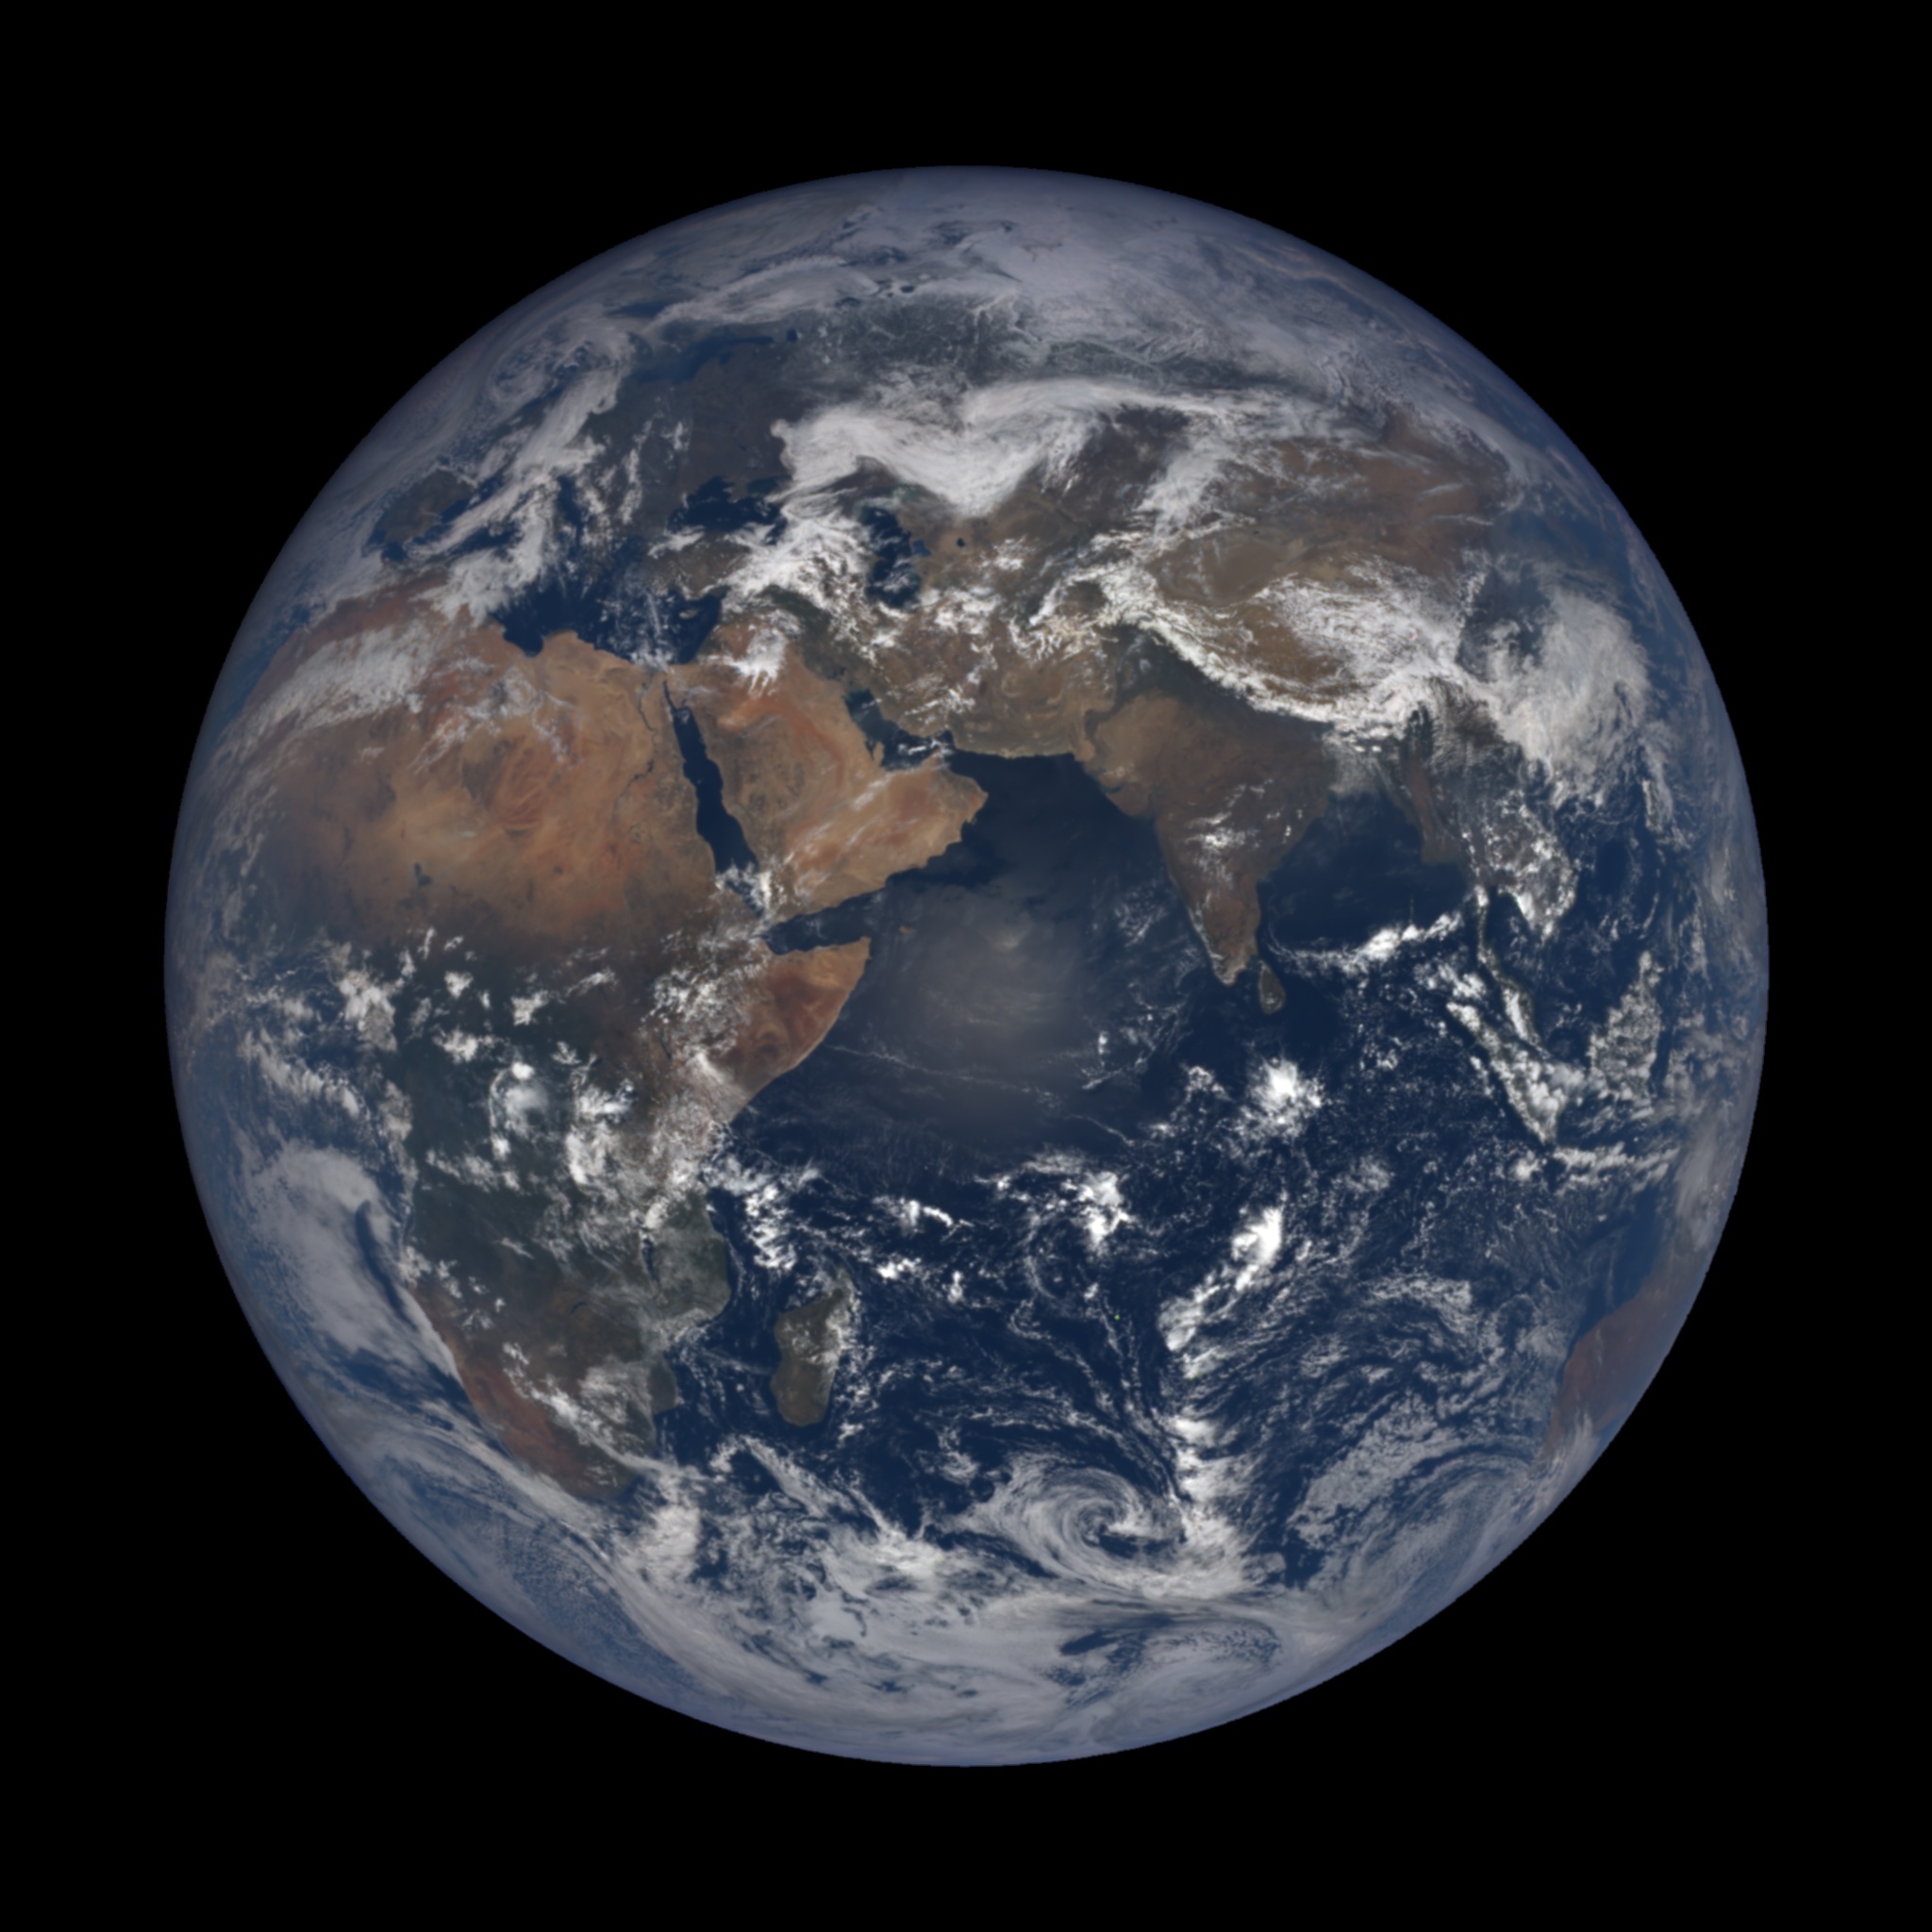
\includegraphics[width=5cm]{images/epic1}
			%\includegraphics[width=7cm]{images/fdl}
		\end{columns}
	\end{center}
	
	\vfill
\end{frame}
}

\begin{frame}
\frametitle{System Earth}

\begin{columns}

\column{.5\textwidth}

{
	%		The Earth is a complex system.
	%		Only some components is observable by 
	%		\begin{itemize}
	%			\item satellite-based or
	%			\item in-situ observations
	%		\end{itemize}
	%		
	
	%	\begin{equation*}\V{y} = f({\M{X}})\end{equation*}
	%	partially observe the complex system Earth
	\textbf{Partially measuring} System Earth
	{\Huge
		\begin{center}
			\begin{tikzpicture}[remember picture]
			\node[draw=none, rounded corners](eo){$\M{X} = \sat\left({\earth}\right)$};
			\end{tikzpicture}
		\end{center}
	}
	
	\vspace{1em}
	\textbf{knowledge extraction} through pattern recognition and machine learning
	
	{\Huge
		\begin{center}
			\begin{tikzpicture}[remember picture]
			\node[draw=none, rounded corners](ml){$\V{?} = f({\M{X}})$};
			\end{tikzpicture}
		\end{center}
	}
	
}

\column{.5\textwidth}

\begin{tikzpicture}[xscale=3, yscale=2]
\node(earth) at (0,0) {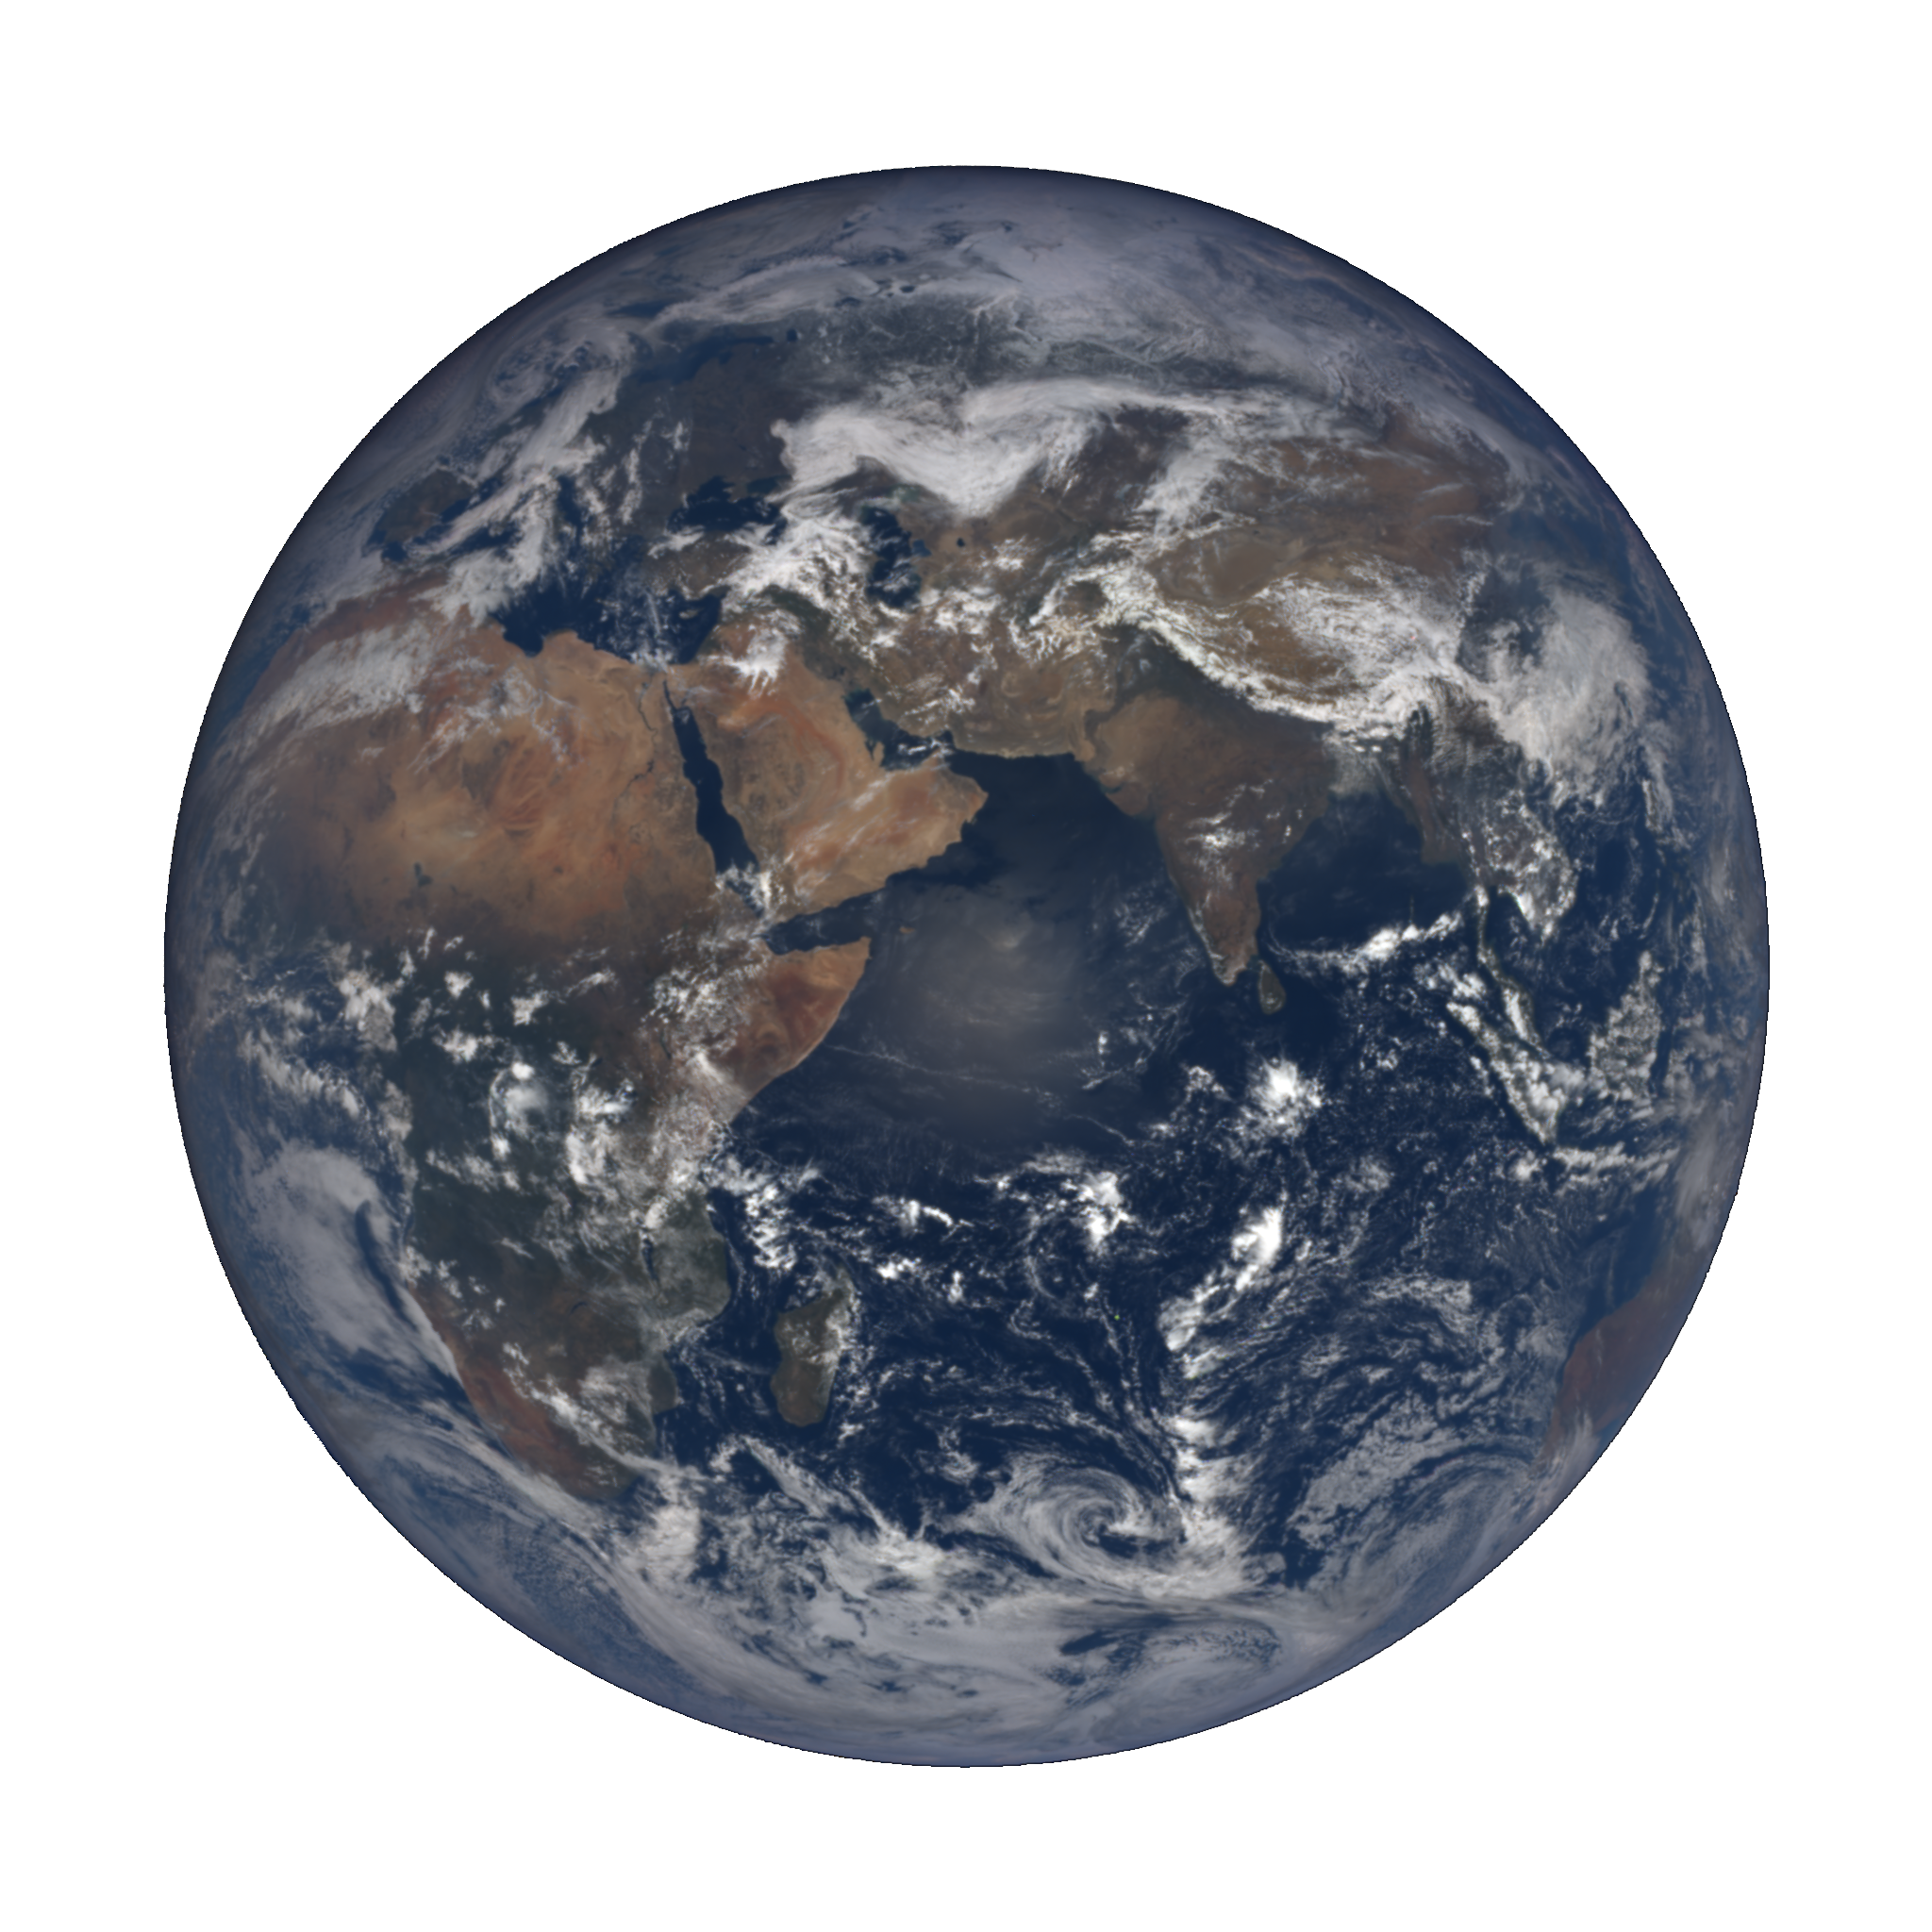
\includegraphics[width=7cm]{images/epicw1}};	

\end{tikzpicture}




\end{columns}


\begin{tikzpicture}[remember picture,overlay]
%\draw (0,1) to[grid with coordinates] (10,7);
\visible<2->{
\node[fill=tumbluedark, text=white, font=\Large, rounded corners](annoteo) at (7,6){Earth Observation Research};
\draw[annot] (annoteo.west)  to[bend right] (sat);
}

\visible<3->{
\node[fill=tumbluedark, text=white, font=\Large, rounded corners](annotml) at (7,3.5){Machine Learning Research};
\draw[annot] (annotml.west)  to[bend right] (ml);
}

\end{tikzpicture}


\end{frame}

\begin{frame}
\frametitle{Going Big...}

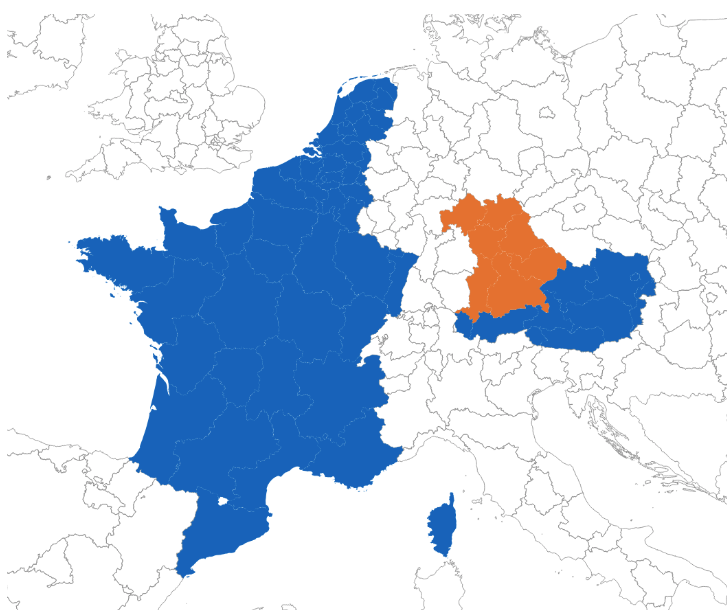
\includegraphics[width=5cm]{images/EuroCrops}
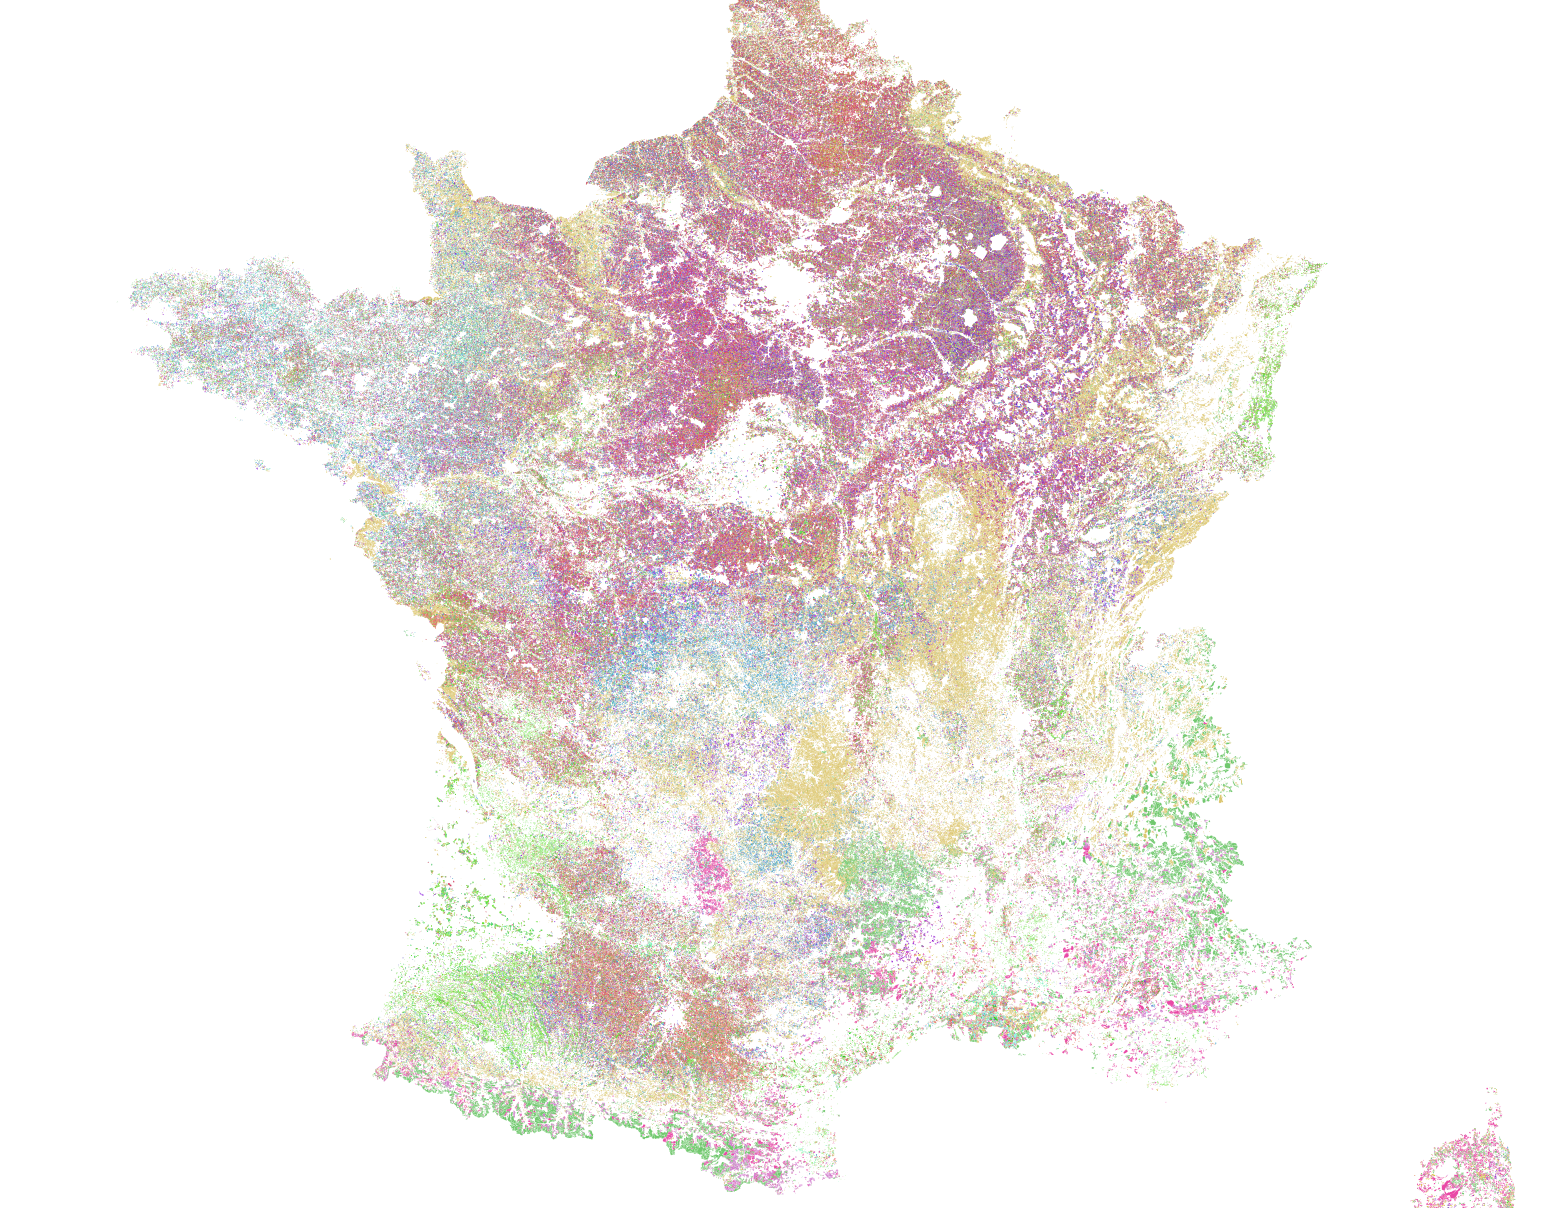
\includegraphics[width=5cm]{images/France}
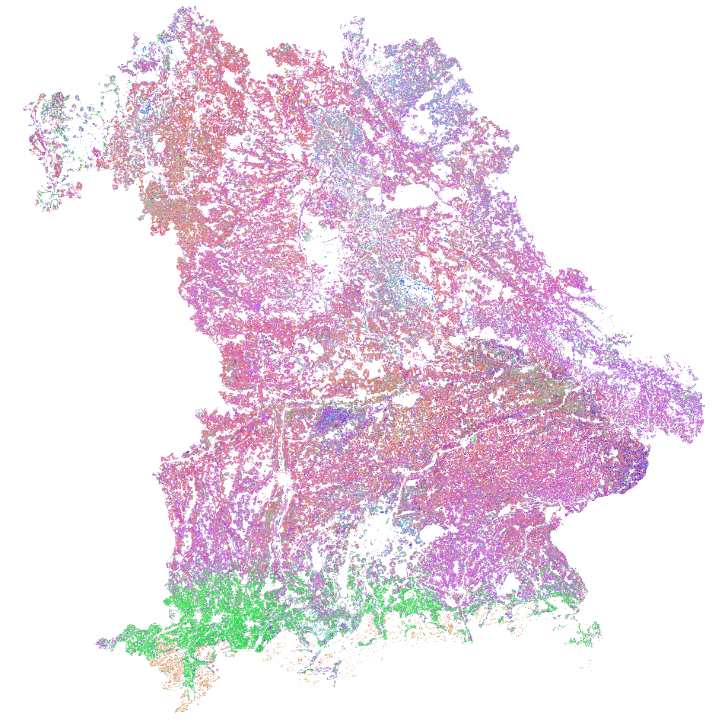
\includegraphics[width=4cm]{images/Bavaria}

\end{frame}

\begin{frame}
\frametitle{Supported by Google Research Credits}


\includegraphics[width=.3\textwidth]{images/google_research_credits}

\includegraphics[width=.3\textwidth]{images/google}

\includegraphics[width=.2\textwidth]{images/earth-engine-logo}
%\includegraphics[width=3cm]{images/250px-Google-Cloud-Storage-Logo}
%\includegraphics[width=3cm]{images/Google_Compute_Engine_logo}
%\includegraphics[width=3cm]{images/google_cloud_sql}


\end{frame}


\begin{frame}
\frametitle{Augmenting Classification Models}

\begin{columns}
	
	\column{.5\textwidth}
	\begin{center}
		
		\begin{tikzpicture}[node distance=1em and 1.5em]
\node[](x0){$x_t$};
\node[rnn, below=of x0](h0){\small$f\left(\xuptot\right)$};
\node[below right= 2em and .0em of h0](y0){$\yhat_t$};
\node[rnn, left=2em of h0,draw=lightgray](hprev){};
\node[rnn, right=2em of h0,draw=lightgray](hnext){};

\draw[infer] (x0) -- (h0);
\draw[infer,draw=lightgray] (hprev) -- (h0);
\draw[infer,draw=lightgray] (h0) -- (hnext);
\draw[infer] (h0) -- (y0) node[midway,right, text=black](wc){$\theta_{cl}$};

\visible<2->{
\node[below left= 2em and .0em of h0](d0){$\delta_t$};
\draw[infer] (h0) -- (d0) node[midway,left, text=black](wd){$\theta_{\delta}$};
}

\visible<3->{
	\node[loss, below=of y0](L0){$\mathcal{L}_{cl}(\yhat,\V{y})$};
	%\node[right=of L0](t0){$\V{y}_t$};
	\draw[-stealth, grad] (y0) -- (L0);
	%\draw[-stealth, grad] (t0) -- (L0);
	%\draw[-stealth, grad] (L0) to [in=-25, out=25, looseness=2] node[midway, right, text=colortrain]{$\frac{\partial\mathcal{L}_{cl}}{\partial\theta_\text{rnn}}$}
	%(h0);
	
	\draw[-stealth, grad] (L0) to [bend right=30] node[near end, right, text=colortrain]{$\frac{\partial\mathcal{L}_{cl}}{\partial\theta_\text{cl}}$}
	(wc);
}

\only<4>{
\node[below=7em of h0, loss](L){$\mathcal{L}(\V{y_t},\yhat_t) = \delta_t\mathcal{L}_{cl}(\V{y_t},\yhat_t)$};
\draw[infer] (L0) -- (L);
\draw[infer] (d0) -- (L);

\draw[-stealth, grad] (L) to [bend right=30] node[midway, right, text=colortrain]{$\frac{\partial\mathcal{L}}{\partial\mathcal{L}_{cl}}$}
(L0);

\draw[-stealth, grad] (L) to [bend left=30] node[midway, left, text=colortrain]{$\frac{\partial\mathcal{L}}{\partial\theta_\delta}$}
(wd);

}

\only<5->{

\node[below=of d0](pt){$P(t)$};
\node[below=8em of h0, loss](L){$\mathcal{L}(\V{y_t},\yhat_t) = P(t)\mathcal{L}_{cl}(\V{y_t},\yhat_t)$};


\draw[infer] (L0) -- (L);
\draw[infer] (d0) -- (pt);
\draw[infer] (pt) -- (L);

%}
%
%\only<6->{
%\node[left=.5em of pt](budget){\small $\prod_{t'<t}(1-\delta_{t'})$};
%\draw[infer] (budget) -- (pt);

%\only<7->{
%	\node[left=.5em of pt](budget){$\mathcal{B}_{t-1}$};
%	
%}

\draw[-stealth, grad] (L) to [bend right=30] node[midway, right, text=colortrain]{$\frac{\partial\mathcal{L}}{\partial\mathcal{L}_{cl}}$}
(L0);

\draw[-stealth, grad] (L) to [bend left=30] node[midway, left, text=colortrain]{$\frac{\partial\mathcal{L}}{\partial P(t)}$}
(pt);

\draw[-stealth, grad] (pt) to [bend left=30] node[midway, left, text=colortrain]{$\frac{\partial P(t)}{\partial \theta_{\delta}}$}
(wd);

}

\end{tikzpicture}

	\end{center}
	\column{.5\textwidth}
	\begin{tikzpicture}

\pgfplotstableread[col sep = comma]{images/qualitative_example/early_rnn_run-sample0.csv}\mydata

\begin{groupplot}[
	group style={
		group name=my plots,
		group size=1 by 5,
		columns=1,
		xlabels at=edge bottom,
		xticklabels at=edge bottom,
		vertical sep=5pt,
	},
	ylabel near ticks,
	ylabel style={rotate=-90},
	width=\textwidth,
	height=3cm,
	axis x line=bottom,
	axis y line=left,
	enlarge x limits=0.01,
	ymajorgrids,
]

\nextgroupplot[no marks, enlarge y limits=0.05, hide x axis, ylabel={$x$}]
\addplot[thick, tumblue] table[x=t, y=x]{\mydata};

\nextgroupplot[no marks, ylabel={$\yhat_t$}, enlarge y limits=0.05, hide x axis]	
\addplot[thick,colorclassone, name path=y1] table[x=t, y=y1]{\mydata};
\addplot[thick,colorclasstwo, name path=y2] table[x=t, y=y2]{\mydata};
\addplot[thick,colorclassthree, name path=y3] table[x=t, y=y3]{\mydata};
\addplot[thick,colorclassfour, name path=y4] table[x=t, y=y4]{\mydata};

%\addplot[colorblue!20] fill between[of = y1 and axis];
%\addplot[colorhgray!20] fill between[of = y2 and axis];
%\addplot[colorgreen!20] fill between[of = y3 and axis];
%\addplot[colororange!20] fill between[of = y4 and axis];
\only<2->{
\nextgroupplot[ybar, bar width=1pt, ylabel={$\delta_t$}]
\addplot[draw=none, fill=tumblue] table[x=t, y=dt]{\mydata};
}

\only<5->{
\nextgroupplot[ybar, bar width=1pt, hide x axis, ylabel={$P(t)$}]
\addplot[draw=none, fill=tumblue] table[x=t, y=pts]{\mydata};

%\nextgroupplot[ybar, bar width=1pt, hide x axis, ylabel={$\prod_{t'<t}(1-\delta_{t'})$}]
%\addplot[draw=none, fill=tumblue, xlabel={time $t$}] table[x=t, y=Bt]{\mydata};
}

\end{groupplot}

\end{tikzpicture}

	
	
\end{columns}

\end{frame}


%\begin{frame}
%	\frametitle{Autoregressive Classification Model}
%	
%	\begin{tikzpicture}[node distance=1em and 2em]

\node[](x0){$x_0$};
\node[rnn, below=of x0](h0){\small$\theta$};
\node[below=of h0](y0){$\yhat_0$};

\node[left=of x0, anchor=east]{\small inputs $x_t$};
\node[left=of h0, anchor=east]{\small model $f(\xuptot;\theta)$};
\node[left=of y0, anchor=east]{\small predictions $y_t$};

\node[right=of x0](x1){$x_1$};
\node[rnn, below=of x1](h1){\small$\theta$};
\node[below=of h1](y1){$\yhat_1$};

\node[right=of x1](x2){$x_2$};
\node[rnn, below=of x2](h2){\small$\theta$};
\node[below=of h2](y2){$\yhat_2$};

\node[right=of x2](x3){$x_3$};
\node[rnn, below=of x3](h3){\small$\theta$};
\node[below=of h3](y3){$\yhat_3$};

\node[right=of x3](x4){$\dots$};
\node[right=of h3](h4){};
\node[right=of y3](y4){$\dots$};

\draw[infer] (h0) -- (h1);
\draw[infer] (h1) -- (h2);
\draw[infer] (h2) -- (h3);
\draw[infer] (h3) -- (h4);

\visible<2->{
	\node[below=of y0](t0){$y_0$};
	\node[below=of y1](t1){$y_1$};
	\node[below=of y2](t2){$y_2$};
	\node[below=of y3](t3){$y_3$};
	\node[left=of t0, anchor=east]{\small labels};
}

\foreach \i in {0,...,3}
{
	\draw[infer] (x\i) -- (h\i);
	\draw[infer] (h\i) -- (y\i);
	
	\visible<2->{
		\draw[stealth-stealth, grad] (y\i) -- node[midway,left](L\i){\small $\mathcal{L}_\i$} (t\i);
	}
	\visible<3->{
		\draw[grad, -stealth](L\i) to [bend left=30] node[midway, left, text=colortrain]{$\frac{\partial\mathcal{L}_\i}{\partial\theta}$} (h\i);
	}
}
\end{tikzpicture}

%	
%\end{frame}


\begin{frame}
\frametitle{Early Classification on Remote Sensing Data}
\begin{tikzpicture}
	
	\tikzstyle{annot} = [font=\tiny\sffamily, text=tumblue]
	\tikzstyle{point} = [thin, tumbluelight, shorten >= .25em, shorten <= .25em]
	
	% from /home/marc/projects/EV2019/images/example/tstop.txt
	\def\tstopv{0.6285714285714286}
	\def\class{winter barley}
	
	\begin{groupplot}[
	group style={
		group name=my plots,
		group size=1 by 2,
		columns=1,
		xlabels at=edge bottom,
		xticklabels at=edge bottom,
		vertical sep=1em,
	},
	ylabel near ticks,
	ylabel style={font=\sffamily\small, rotate=-90},
	width=\textwidth,
	height=4cm,
	axis x line=bottom,
	axis y line=left,
	enlarge x limits=0.01,
	xtick={0,0.25,0.5,0.75,1},
	xticklabels={January,April,June,Sepember,December},
	ymajorgrids,
	ymin=0, ymax=1.4
	]
	
	\nextgroupplot[thin,
		no marks,  
		ylabel={$\V{x}$},
		draw opacity=.8,
		smooth,
		legend columns=4,
		legend style={at={(.5,1)},anchor=south, line width=1pt, fill=tumblue!10}
		]
		 
	\addplot[b1color] table [x=t, y=B1, col sep=comma, forget plot] {images/example/input.csv};
	\addplot[b9color] table [x=t, y=B9, col sep=comma, forget plot] {images/example/input.csv};
	\addplot[b10color] table [x=t, y=B10, col sep=comma] {images/example/input.csv};
	
	\addplot[b11color] table [x=t, y=B11, col sep=comma, forget plot] {images/example/input.csv};
	\addplot[b12color] table [x=t, y=B12, col sep=comma] {images/example/input.csv};
	
	\addplot[b5color] table [x=t, y=B5, col sep=comma, forget plot] {images/example/input.csv};
	\addplot[b6color] table [x=t, y=B6, col sep=comma, forget plot] {images/example/input.csv};
	\addplot[b7color] table [x=t, y=B7, col sep=comma, forget plot] {images/example/input.csv};
	\addplot[b8color] table [x=t, y=B8, col sep=comma, forget plot] {images/example/input.csv};
	\addplot[b8Acolor] table [x=t, y=B8A, col sep=comma] {images/example/input.csv};
		
	\addplot[b2color] table [x=t, y=B2, col sep=comma, forget plot] {images/example/input.csv};
	\addplot[b3color] table [x=t, y=B3, col sep=comma, forget plot] {images/example/input.csv};
	\addplot[b4color] table [x=t, y=B4, col sep=comma] {images/example/input.csv};
	
	
	\draw[fill=white, draw=none, opacity=.5] (axis cs:\tstopv,0) rectangle (axis cs:1,1.1);
	
	\node[annot](cllab) at (axis cs:.2,1.3) {clouds (noise)};
	\draw[point] (cllab) -- (axis cs:.13,.7);
	\draw[point] (cllab) -- (axis cs:.25,.7);
	\draw[point] (cllab) -- (axis cs:.53,1);
	\draw[point] (cllab) -- (axis cs:.45,.85);
	
	\node[annot](glab) at (axis cs:.8,1.3) {ground (signal)};
	\draw[point] (glab) -- (axis cs:.38,.3);
	\draw[point] (glab) -- (axis cs:.21,.3);
	\draw[point] (glab) -- (axis cs:.7,.3);
	
	\draw (axis cs:\tstopv,0) -- (axis cs:\tstopv,1) node[above]{$\tstop$};
	
	
	
	\legend{3 atmospheric, 2 short-wave infrared, 5 near infrared, 3 visible bands}
	
	\nextgroupplot[thin,
		smooth,
		no marks, 
		ylabel={$\yhat$},
		legend style={at={(.5,-.2)},anchor=north, line width=1pt, fill=tumblue!10},
		legend columns=6]	
	
	\addplot[meadowcolor] table [x=t, y=meadows, col sep=comma] {images/example/proba.csv};
	\addplot[wbarleycolor, thick] table [x=t, y=winter barley, col sep=comma] {images/example/proba.csv};
	\addplot[corncolor] table [x=t, y=corn, col sep=comma] {images/example/proba.csv};
	\addplot[wheatcolor,] table [x=t, y=winter wheat, col sep=comma] {images/example/proba.csv};
	\addplot[sbarleycolor] table [x=t, y=summer barley, col sep=comma] {images/example/proba.csv};
	\addplot[clovercolor] table [x=t, y=clover, col sep=comma] {images/example/proba.csv};
	\addplot[triticalecolor] table [x=t, y=winter triticale, col sep=comma] {images/example/proba.csv};
	
	\draw[fill=white, draw=none, opacity=.5] (axis cs:\tstopv,0) rectangle (axis cs:1,1);
	
	\draw (axis cs:\tstopv,0) -- (axis cs:\tstopv,2.2);
	
	\node[annot](rand) at (axis cs:.1,.8) {first hints};
	\draw[point] (rand) -- (axis cs:.2,.15);
	
	\node[annot](wrong) at (axis cs:.17,1.1) {initially wrong predictions};
	\draw[point] (wrong) -- (axis cs:.25,.7);
	\draw[point] (wrong) -- (axis cs:.4,1);
	
	\node[annot, align=center](corrwait) at (axis cs:.4,1.3) {waiting for more data};
	\draw[point] (corrwait) -- (axis cs:.5,.8);
	
	\node[annot](corr) at (axis cs:.8,1.3) {seen enough data};
	\draw[point] (corr) -- (axis cs:.63,1);
	
	\legend{meadows,\textbf{winter barley},corn,winter wheat,summer barley,clover,winter triticale}
	
	
%	\addplot[thick,colorclassone, name path=y1] table[x=t, y=y1]{\mydata};
%	\addplot[thick,colorclasstwo, name path=y2] table[x=t, y=y2]{\mydata};
%	\addplot[thick,colorclassthree, name path=y3] table[x=t, y=y3]{\mydata};
%	\addplot[thick,colorclassfour, name path=y4] table[x=t, y=y4]{\mydata};
	%\addplot[colorblue!20] fill between[of = y1 and axis];
	%\addplot[colorhgray!20] fill between[of = y2 and axis];
	%\addplot[colorgreen!20] fill between[of = y3 and axis];
	%\addplot[colororange!20] fill between[of = y4 and axis];
	
	
	\end{groupplot}
	
	\end{tikzpicture}

\url{https://arxiv.org/abs/1901.10681}


\end{frame}


\begin{frame}
\frametitle{Multi-Layer RNN baseline}

\newcommand{\confmat}[3]{

\begin{tikzpicture}

  \def\vmax{#3}
  \def\dataindex{#2}
  
%
%  \pgfplotsset{every axis label/.append style={font=\footnotesize},tick pos=right, ylabel near ticks}
%  
%  \pgfplotsset{
%    axis line style={%
%      opacity=0 
%    }   
%  }

  \begin{groupplot}[
  	group style={
  		group size=2 by 1,
  		xlabels at=edge bottom,
  		ylabels at=edge left,
  		xticklabels at=edge bottom,
  		vertical sep=35pt,
  		group name=seq_len_plot
  	},
  	axis line style={draw=none},
  	title style={yshift=.75em,},
    width=6cm,
    height=6cm,
    enlargelimits=false,
    xtick=data,
%     ymin=1,
    xtick distance=1,
    ytick distance=1,
    colormap={example}{%
		color=(tumwhite)%color=(tumbluelight)
%		color=(tumivory)
%		color=(tumorange)
		color=(tumblue)%color=(tumbluelight)
%		color=(tumblack)
	},
    ytick=data,
    ytick align=outside,
    xtick align=outside,
%    tick style={draw=none},
    ytick pos = left,  
    tick label style = {font=\tiny\sansmath\sffamily},
    %xticklabel = {xshift=-0.75cm}
    yticklabel pos=left,
    %yticklabel near ticks,
    xlabel={\normalsize predicted},
    xlabel style={yshift=1em},
    ylabel style={yshift=-3em},
    x label style={at={(axis description cs:0.5,1)},anchor=south},
    y label style={at={(axis description cs:-0.1,.5)},anchor=south},
    ylabel={\normalsize ground truth},
%     ylabel near ticks,
%    xticklabels={},
  ]
  \nextgroupplot[
%      yticklabels={
%%      	{sugar beet},
%%      	{summer oat},
%%      	{meadow},
%%      	{rape},
%%      	%{vegetable},
%%      	{hop},
%%      	{winter spelt},
%%      	{winter triticale},
%%      	{beans},
%%      	{peas},
%%      	{potato},
%%      	{soybeans},
%%      	{asparagus},
%%      	{winter wheat},
%%      	{winter barley},
%%      	{winter rye},
%%      	{summer barley},
%%      	{maize}
%      },
%      xticklabels={
%%      	{sug.},
%%      	{s. oat},
%%      	{mead.},
%%      	{rape},
%%      	%{vegetable},
%%      	{hop},
%%      	{w. spelt},
%%      	{w. trit.},
%%      	{beans},
%%      	{peas},
%%      	{potato},
%%      	{soyb.},
%%      	{asp.},
%%      	{w. wheat},
%%      	{w. barley},
%%      	{w. rye},
%%      	{s. barley},
%%      	{maize}
%      },
     %colorbar style={title={\precisionrecall}, xshift=0cm, font=\footnotesize},
     colorbar right,
     colorbar style={
        	title={}, 
        	font=\footnotesize,
        	%at={(0,1)},
        	anchor=north west,
        	width=8pt,
        	ticklabel pos=right,
        	ticklabel style={xshift=2em},
%        	label style={yshift=-1em},
        	rounded corners=1pt
     },
  ]
  
    \addplot[
      matrix plot,
%      draw=tumwhite,
%       nodes near coords=\coordindex,
%       nodes near coords align={center},
%       nodes near coords style={font=\scriptsize},
        shader=faceted,
        faceted color=tumgraylight!20,
%       shader=faceted interp,
      mesh/cols=13,
      empty line=scanline,
      point meta=explicit,
      point meta min=0,
      point meta max=\vmax,
    ] table[meta index=\dataindex] {#1};
%   \nextgroupplot[
%       title=2017,
%       %colorbar style={title={\precisionrecall}, xshift=0cm, font=\footnotesize},
%       colorbar right,
%       colorbar style={
%       	title={a}, 
%       	font=\footnotesize,
%       	%at={(0,1)},
%       	anchor=north west,
%       	width=8pt,
%       	ticklabel pos=right,
%       	ticklabel style={xshift=1em},
%       	label style={yshift=1em},
%       	rounded corners=1pt
%       },
%       yticklabels={},
%     xticklabels={
%           	{sug.},
%           	{s. oat},
%           	{mead.},
%           	{rape},
%           	%{vegetable},
%           	{hop},
%           	{w. spelt},
%           	{w. trit.},
%           	{beans},
%           	{peas},
%           	{potato},
%           	{soyb.},
%           	{asp.},
%           	{w. wheat},
%           	{w. barley},
%           	{w. rye},
%           	{s. barley},
%           	{maize}
%     },
%       ]
%    
%    \addplot[
%    matrix plot,
%%    draw=tumwhite,
%    ,   
%    %       nodes near coords=\coordindex,
%    %       nodes near coords align={center},
%    %       nodes near coords style={font=\scriptsize},
%    shader=faceted,
%    faceted color=tumgraylight,
%    %       shader=faceted interp,
%    mesh/cols=17,
%    empty line=scanline,
%    point meta=explicit,
%    point meta min=0,
%    point meta max=\vmax,
%    ] table[meta index=\dataindex] {images/confmat/formatted_grucm2017.csv};
    
  \end{groupplot}
\end{tikzpicture}
}

\begin{columns}
	
	\column{.5\textwidth}
	\textbf{Precision}
	
	\confmat{images/data/BreizhCrops_rnn/npy/confmat_flat.csv}{3}{1}
	
	\column{.5\textwidth}
	\textbf{Recall}
	
	\confmat{images/data/BreizhCrops_rnn/npy/confmat_flat.csv}{4}{1}
	
\end{columns}

\end{frame}

\begin{frame}
\frametitle{Transformer baseline}

\newcommand{\confmat}[3]{

\begin{tikzpicture}

  \def\vmax{#3}
  \def\dataindex{#2}
  
%
%  \pgfplotsset{every axis label/.append style={font=\footnotesize},tick pos=right, ylabel near ticks}
%  
%  \pgfplotsset{
%    axis line style={%
%      opacity=0 
%    }   
%  }

  \begin{groupplot}[
  	group style={
  		group size=2 by 1,
  		xlabels at=edge bottom,
  		ylabels at=edge left,
  		xticklabels at=edge bottom,
  		vertical sep=35pt,
  		group name=seq_len_plot
  	},
  	axis line style={draw=none},
  	title style={yshift=.75em,},
    width=6cm,
    height=6cm,
    enlargelimits=false,
    xtick=data,
%     ymin=1,
    xtick distance=1,
    ytick distance=1,
    colormap={example}{%
		color=(tumwhite)%color=(tumbluelight)
%		color=(tumivory)
%		color=(tumorange)
		color=(tumblue)%color=(tumbluelight)
%		color=(tumblack)
	},
    ytick=data,
    ytick align=outside,
    xtick align=outside,
%    tick style={draw=none},
    ytick pos = left,  
    tick label style = {font=\tiny\sansmath\sffamily},
    %xticklabel = {xshift=-0.75cm}
    yticklabel pos=left,
    %yticklabel near ticks,
    xlabel={\normalsize predicted},
    xlabel style={yshift=1em},
    ylabel style={yshift=-3em},
    x label style={at={(axis description cs:0.5,1)},anchor=south},
    y label style={at={(axis description cs:-0.1,.5)},anchor=south},
    ylabel={\normalsize ground truth},
%     ylabel near ticks,
%    xticklabels={},
  ]
  \nextgroupplot[
%      yticklabels={
%%      	{sugar beet},
%%      	{summer oat},
%%      	{meadow},
%%      	{rape},
%%      	%{vegetable},
%%      	{hop},
%%      	{winter spelt},
%%      	{winter triticale},
%%      	{beans},
%%      	{peas},
%%      	{potato},
%%      	{soybeans},
%%      	{asparagus},
%%      	{winter wheat},
%%      	{winter barley},
%%      	{winter rye},
%%      	{summer barley},
%%      	{maize}
%      },
%      xticklabels={
%%      	{sug.},
%%      	{s. oat},
%%      	{mead.},
%%      	{rape},
%%      	%{vegetable},
%%      	{hop},
%%      	{w. spelt},
%%      	{w. trit.},
%%      	{beans},
%%      	{peas},
%%      	{potato},
%%      	{soyb.},
%%      	{asp.},
%%      	{w. wheat},
%%      	{w. barley},
%%      	{w. rye},
%%      	{s. barley},
%%      	{maize}
%      },
     %colorbar style={title={\precisionrecall}, xshift=0cm, font=\footnotesize},
     colorbar right,
     colorbar style={
        	title={}, 
        	font=\footnotesize,
        	%at={(0,1)},
        	anchor=north west,
        	width=8pt,
        	ticklabel pos=right,
        	ticklabel style={xshift=2em},
%        	label style={yshift=-1em},
        	rounded corners=1pt
     },
  ]
  
    \addplot[
      matrix plot,
%      draw=tumwhite,
%       nodes near coords=\coordindex,
%       nodes near coords align={center},
%       nodes near coords style={font=\scriptsize},
        shader=faceted,
        faceted color=tumgraylight!20,
%       shader=faceted interp,
      mesh/cols=13,
      empty line=scanline,
      point meta=explicit,
      point meta min=0,
      point meta max=\vmax,
    ] table[meta index=\dataindex] {#1};
%   \nextgroupplot[
%       title=2017,
%       %colorbar style={title={\precisionrecall}, xshift=0cm, font=\footnotesize},
%       colorbar right,
%       colorbar style={
%       	title={a}, 
%       	font=\footnotesize,
%       	%at={(0,1)},
%       	anchor=north west,
%       	width=8pt,
%       	ticklabel pos=right,
%       	ticklabel style={xshift=1em},
%       	label style={yshift=1em},
%       	rounded corners=1pt
%       },
%       yticklabels={},
%     xticklabels={
%           	{sug.},
%           	{s. oat},
%           	{mead.},
%           	{rape},
%           	%{vegetable},
%           	{hop},
%           	{w. spelt},
%           	{w. trit.},
%           	{beans},
%           	{peas},
%           	{potato},
%           	{soyb.},
%           	{asp.},
%           	{w. wheat},
%           	{w. barley},
%           	{w. rye},
%           	{s. barley},
%           	{maize}
%     },
%       ]
%    
%    \addplot[
%    matrix plot,
%%    draw=tumwhite,
%    ,   
%    %       nodes near coords=\coordindex,
%    %       nodes near coords align={center},
%    %       nodes near coords style={font=\scriptsize},
%    shader=faceted,
%    faceted color=tumgraylight,
%    %       shader=faceted interp,
%    mesh/cols=17,
%    empty line=scanline,
%    point meta=explicit,
%    point meta min=0,
%    point meta max=\vmax,
%    ] table[meta index=\dataindex] {images/confmat/formatted_grucm2017.csv};
    
  \end{groupplot}
\end{tikzpicture}
}

\begin{columns}

\column{.5\textwidth}
\confmat{images/data/BreizhCrops_transformer/npy/confmat_flat.csv}{3}{1}

\column{.5\textwidth}
\confmat{images/data/BreizhCrops_transformer/npy/confmat_flat.csv}{4}{1}

\end{columns}

\end{frame}

